\documentclass[a4paper,12pt]{article}

\usepackage[all]{xy}
\usepackage{amsmath, amsthm, amsfonts, amscd}
\usepackage{bidipoem}
\usepackage{multicol}
\usepackage{makeidx}
\makeindex
\usepackage{subfigure}
\usepackage{graphicx}
\usepackage{xepersian}
\settextfont{IRAmir}

\title{\lr{How to import figures}}
\author{\lr{Alireza Arzehgar}}
\date{}

\begin{document}
\maketitle
\tableofcontents
\listoffigures

سلام سلام بچه ها ۱۲۳۴

% 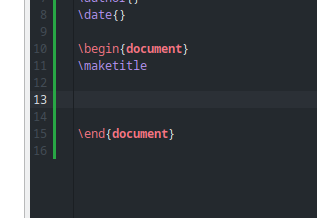
\includegraphics{figs/shot1.png}
% 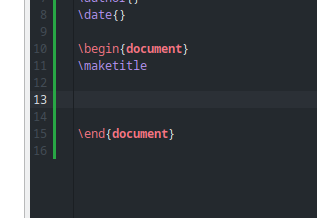
\includegraphics[width = 4cm, height = 4cm]{./figs/shot1.png}
% 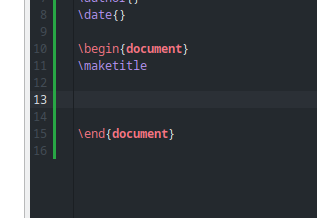
\includegraphics[scale=1.5]{./figs/shot1.png}

\section{shot}
\begin{figure}[h!]
\caption{shotttt}
\label{l1}
 \subfigure[\lr{screen shot1}]{
    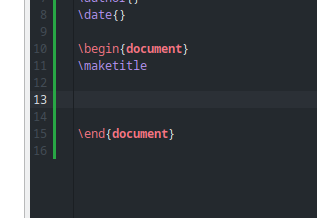
\includegraphics{./figs/shot1.png}
    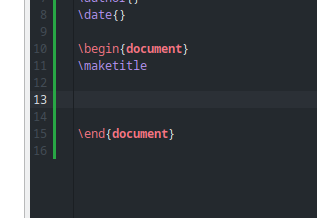
\includegraphics{./figs/shot1.png}
 }
 \subfigure[\lr{Screen shot2}]{
    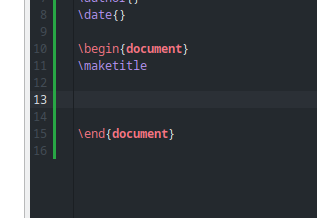
\includegraphics{./figs/shot1.png}
    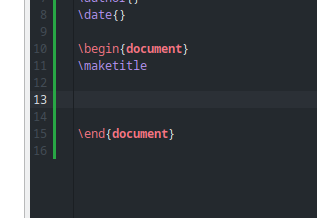
\includegraphics{./figs/shot1.png}
 }
\end{figure}


\begin{traditionalpoem}
تا توانی میگریز از یار بد &
یار بد بد تر بود از مار بد \\
مار بد تنها تو را بر جان زند &
یار بد بر چان و بر ایمان زند \\
\end{traditionalpoem}


\[
 \begin{CD}
  F @>f(x)>g(x)> G\\
  @VVV @AAA\\
  C @<<< D\\
 \end{CD}
\]

\[
\xymatrix{
A \ar[r] & B & \ar[l]^-{f}_{g} C \ar@{.>}[r] & D
}
\]

\begin{multicols}{2}
\begin{align*}
 \underbrace{\int e^x \sin x}_{\romannumeral 1} &= e^x \sin x - e^x \cos x - \int e^x \sin x \\
 \Rightarrow & \ 2 \romannumeral 1 = e^x \sin x - e^x \cos x \\
 \Rightarrow & \  \romannumeral 1 = \tfrac12 e^x (\sin x - \cos x) \\
\end{align*}
\hfill
\columnbreak

\xymatrix{
D & I\\
\sin x \ar[dr]^{+} & e^x\\
\cos x \ar[dr]^{-} & e^x\\
-\sin x & e^x\\
}
\end{multicols}

\end{document}
